\documentclass[11pt, a4paper]{article}

% --- PACKAGES ---
\usepackage[utf8]{inputenc}
\usepackage[T1]{fontenc}
\usepackage{amsmath}         % For advanced math environments (align, etc.)
\usepackage{amssymb}         % For symbols like \mathbb{R}
\usepackage[margin=1in]{geometry} % For reasonable margins
\usepackage{graphicx}        % For including images
\usepackage{amsthm}          % For theorem, definition environments
\usepackage{hyperref}        % For clickable links
\usepackage{booktabs}        % For professional tables
\usepackage{parskip}         % Adds space between paragraphs, no indent

% --- THEOREM ENVIRONMENTS ---
\newtheorem{theorem}{Theorem}[section]
\newtheorem{corollary}[theorem]{Corollary}
\newtheorem{lemma}[theorem]{Lemma}
\theoremstyle{definition}
\newtheorem{definition}[theorem]{Definition}
\newtheorem{example}[theorem]{Example}

% --- HYPERLINK SETUP ---
\hypersetup{
    colorlinks=true,
    linkcolor=blue,
    filecolor=blue,      
    urlcolor=blue,
    citecolor=blue,
}

% --- DOCUMENT TITLE ---
\title{CSE 422: Mathematical Background Review}
\author{Combined from Lecture Notes and Textbook}
\date{October 24, 2025}

% --- BEGIN DOCUMENT ---
\begin{document}

\maketitle

\begin{abstract}
    This document reviews foundational mathematical concepts frequently used in computer science, data science, and engineering. Data science is fundamentally about making decisions under uncertainty, and probability is the mathematical tool for modeling, analyzing, and predicting random events. This review covers topics including functions, polynomials, infinite series (geometric, Taylor), combinatorics (permutations, combinations, binomial theorem), and integration techniques, all of which are essential for this analysis \cite{Chan2021}. This document combines notes originally prepared by Md Shahriar Karim \cite{KarimCSE422} with theoretical background from \cite{Chan2021}.
\end{abstract}

\tableofcontents

\newpage

\section{Functions: Inverses and Properties}

\subsection{Inverse Functions}
A function $f$ is invertible if and only if it is a \textbf{bijection}, meaning it is both:
\begin{itemize}
    \item \textbf{One-to-one (Injective):} Each element in the range is mapped to by at most one element in the domain.
    \item \textbf{Onto (Surjective):} Each element in the range is mapped to by at least one element in the domain.
\end{itemize}
When we invert a function, the range of the original function $f$ becomes the domain for the inverse function $f^{-1}$.

\begin{example}[Finding an Inverse (Note Example)]
Find the inverse of $f(x) = \frac{2}{e^x + 1}$.
Let $y = f(x)$. We solve for $x$:
\begin{align*}
    y &= \frac{2}{e^x + 1} \\
    y(e^x + 1) &= 2 \\
    ye^x + y &= 2 \\
    ye^x &= 2 - y \\
    e^x &= \frac{2-y}{y} \\
    x &= \ln\left(\frac{2-y}{y}\right) = \ln\left(\frac{2}{y} - 1\right)
\end{align*}
Therefore, the inverse function is $f^{-1}(y) = \ln\left(\frac{2}{y} - 1\right)$. Swapping variables to use $x$, we get:
\[
f^{-1}(x) = \ln\left(\frac{2}{x} - 1\right)
\]
\end{example}

\subsection{Checking for One-to-One (Injective)}
A function is one-to-one if $f(x_1) = f(x_2)$ implies $x_1 = x_2$.

\begin{example}[Note Example]
Is $f(x) = \frac{x+5}{x-6}$ one-to-one?
Set $f(x_1) = f(x_2)$:
\begin{align*}
    \frac{x_1+5}{x_1-6} &= \frac{x_2+5}{x_2-6} \\
    (x_1+5)(x_2-6) &= (x_2+5)(x_1-6) \\
    x_1x_2 - 6x_1 + 5x_2 - 30 &= x_1x_2 + 5x_1 - 6x_2 - 30 \\
    -6x_1 + 5x_2 &= 5x_1 - 6x_2 \\
    11x_2 &= 11x_1 \implies x_1 = x_2
\end{align*}
Yes, the function is one-to-one.
\end{example}

A strictly increasing or strictly decreasing function (where $f'(x) > 0$ or $f'(x) < 0$ for all $x$ in the domain) is always one-to-one.

\begin{example}[One-to-one via Derivative (Note Example)]
Is $f(x) = xe^{x^4}$ one-to-one for $x \in \mathbb{R}$?
We check its derivative, $f'(x)$:
\begin{align*}
    f'(x) &= (1) \cdot e^{x^4} + x \cdot (e^{x^4} \cdot 4x^3) \\
    &= e^{x^4} + 4x^4 e^{x^4} \\
    &= e^{x^4} (1 + 4x^4)
\end{align*}
Since $e^{x^4}$ is always positive and $(1 + 4x^4)$ is always positive for any real $x$, $f'(x)$ is always positive.
Because $f'(x) > 0$ for all $x$, the function is strictly increasing, and therefore it is one-to-one.
\end{example}

\section{Polynomials}
A polynomial of degree $n$ is a function of the form:
\[
f(x) = a_n x^n + a_{n-1} x^{n-1} + \dots + a_1 x + a_0
\]
The \textbf{degree} is the highest power of $x$ with a non-zero coefficient.

\subsection{Roots and Multiplicity}
The \textbf{roots} of a polynomial are the values of $x$ for which $f(x) = 0$.

The \textbf{multiplicity} of a root is the number of times it appears as a factor. For example, in $f(x) = (x-2)^3(x+4)^1$, the root $x=2$ has a multiplicity of 3, and the root $x=-4$ has a multiplicity of 1.

The multiplicity of a root provides graphical information:
\begin{itemize}
    \item \textbf{Even multiplicity:} The graph \textbf{touches} the x-axis at the root and turns around.
    \item \textbf{Odd multiplicity:} The graph \textbf{crosses} the x-axis at the root.
\end{itemize}

\begin{example}[Note Example]
Sketch $f(x) = (x-2)^2(x+1)$.
\begin{itemize}
    \item Roots are $x=2$ (multiplicity 2, even) and $x=-1$ (multiplicity 1, odd).
    \item The graph will \textbf{touch} the x-axis at $x=2$.
    \item The graph will \textbf{cross} the x-axis at $x=-1$.
\end{itemize}
\end{example}

\begin{figure}[h!]
  \centering
  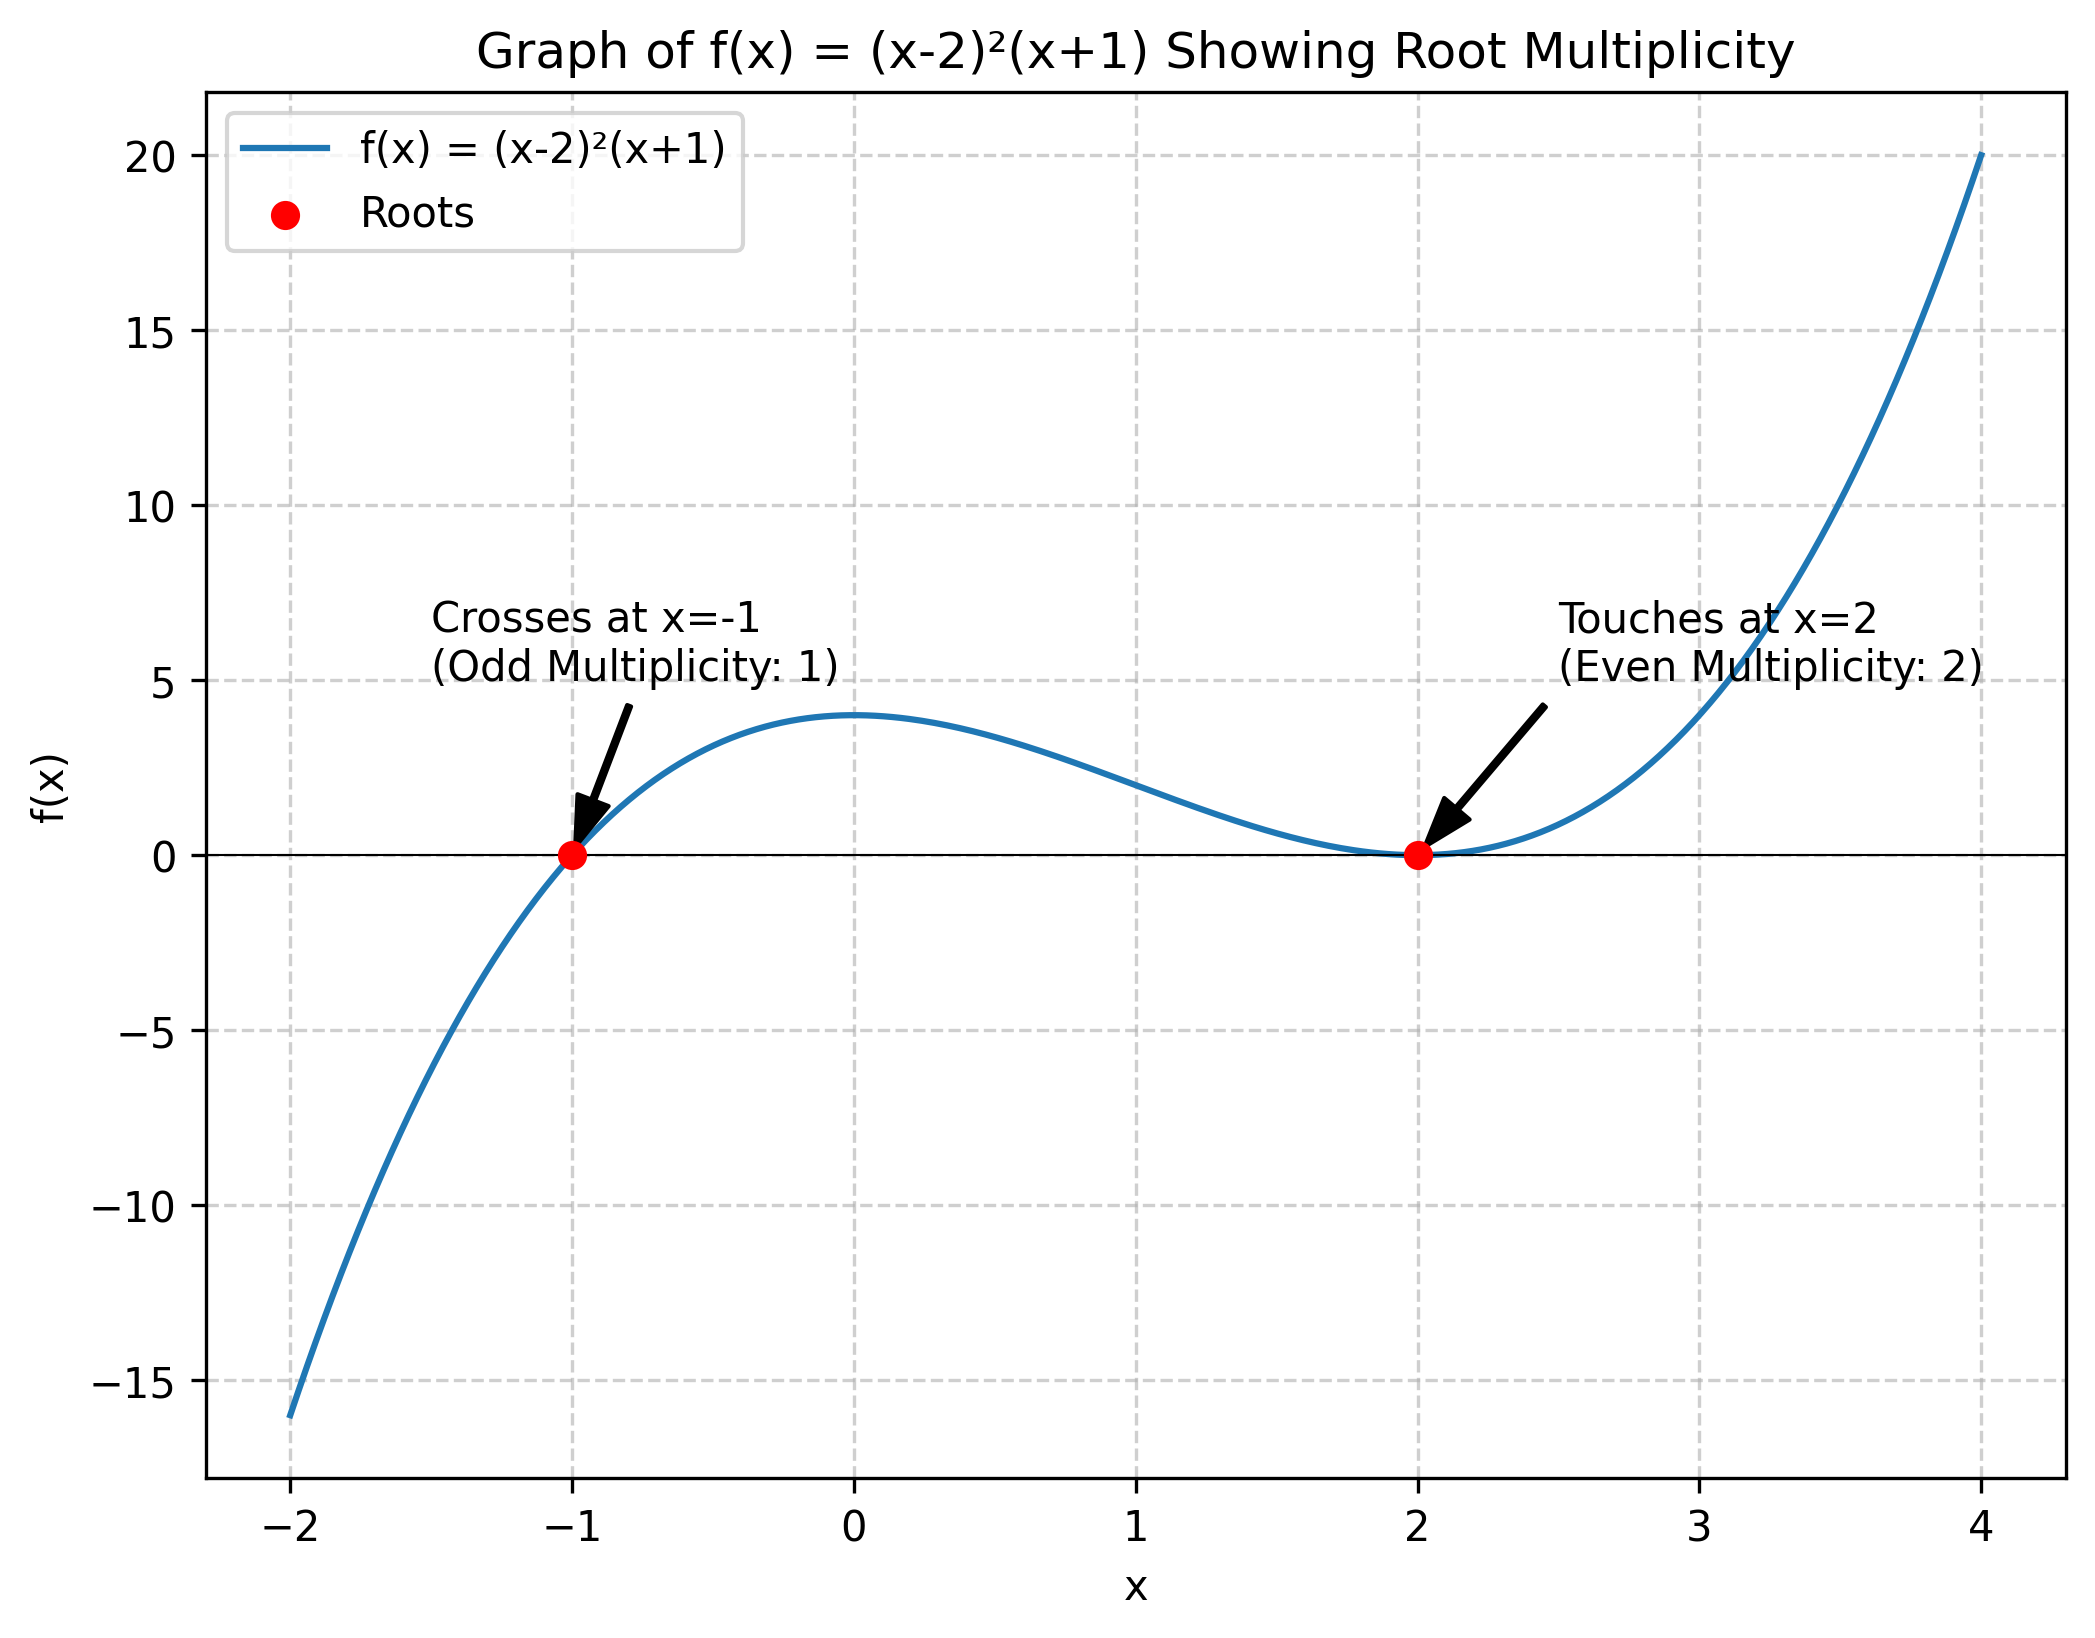
\includegraphics[width=0.8\textwidth]{figure_1_multiplicity.png}
  \caption{Graph showing root multiplicity.}
  \label{fig:multiplicity}
\end{figure}

\newpage
\section{Infinite Series and Approximations}
Infinite series are used frequently in probability, such as when evaluating the expectation and variance of random variables \cite[Sec 1.1]{Chan2021}.

\subsection{Geometric Series}
A geometric series is a sequence where each term after the first is found by multiplying the previous one by a fixed, non-zero number called the \textbf{common ratio}, $r$.

\begin{example}[Motivating Example: Coin Flip \cite{Chan2021}]
Imagine you flip a fair coin until you get a head.
\begin{itemize}
    \item P(1 flip: H) = $\frac{1}{2}$
    \item P(2 flips: TH) = $\frac{1}{2} \times \frac{1}{2} = \frac{1}{4}$
    \item P(3 flips: TTH) = $\frac{1}{2} \times \frac{1}{2} \times \frac{1}{2} = \frac{1}{8}$
\end{itemize}
The sequence of probabilities is $\{\frac{1}{2}, \frac{1}{4}, \frac{1}{8}, \dots\}$, a geometric sequence with first term $a = 1/2$ and common ratio $r = 1/2$.
\end{example}

\begin{figure}[h!]
  \centering
  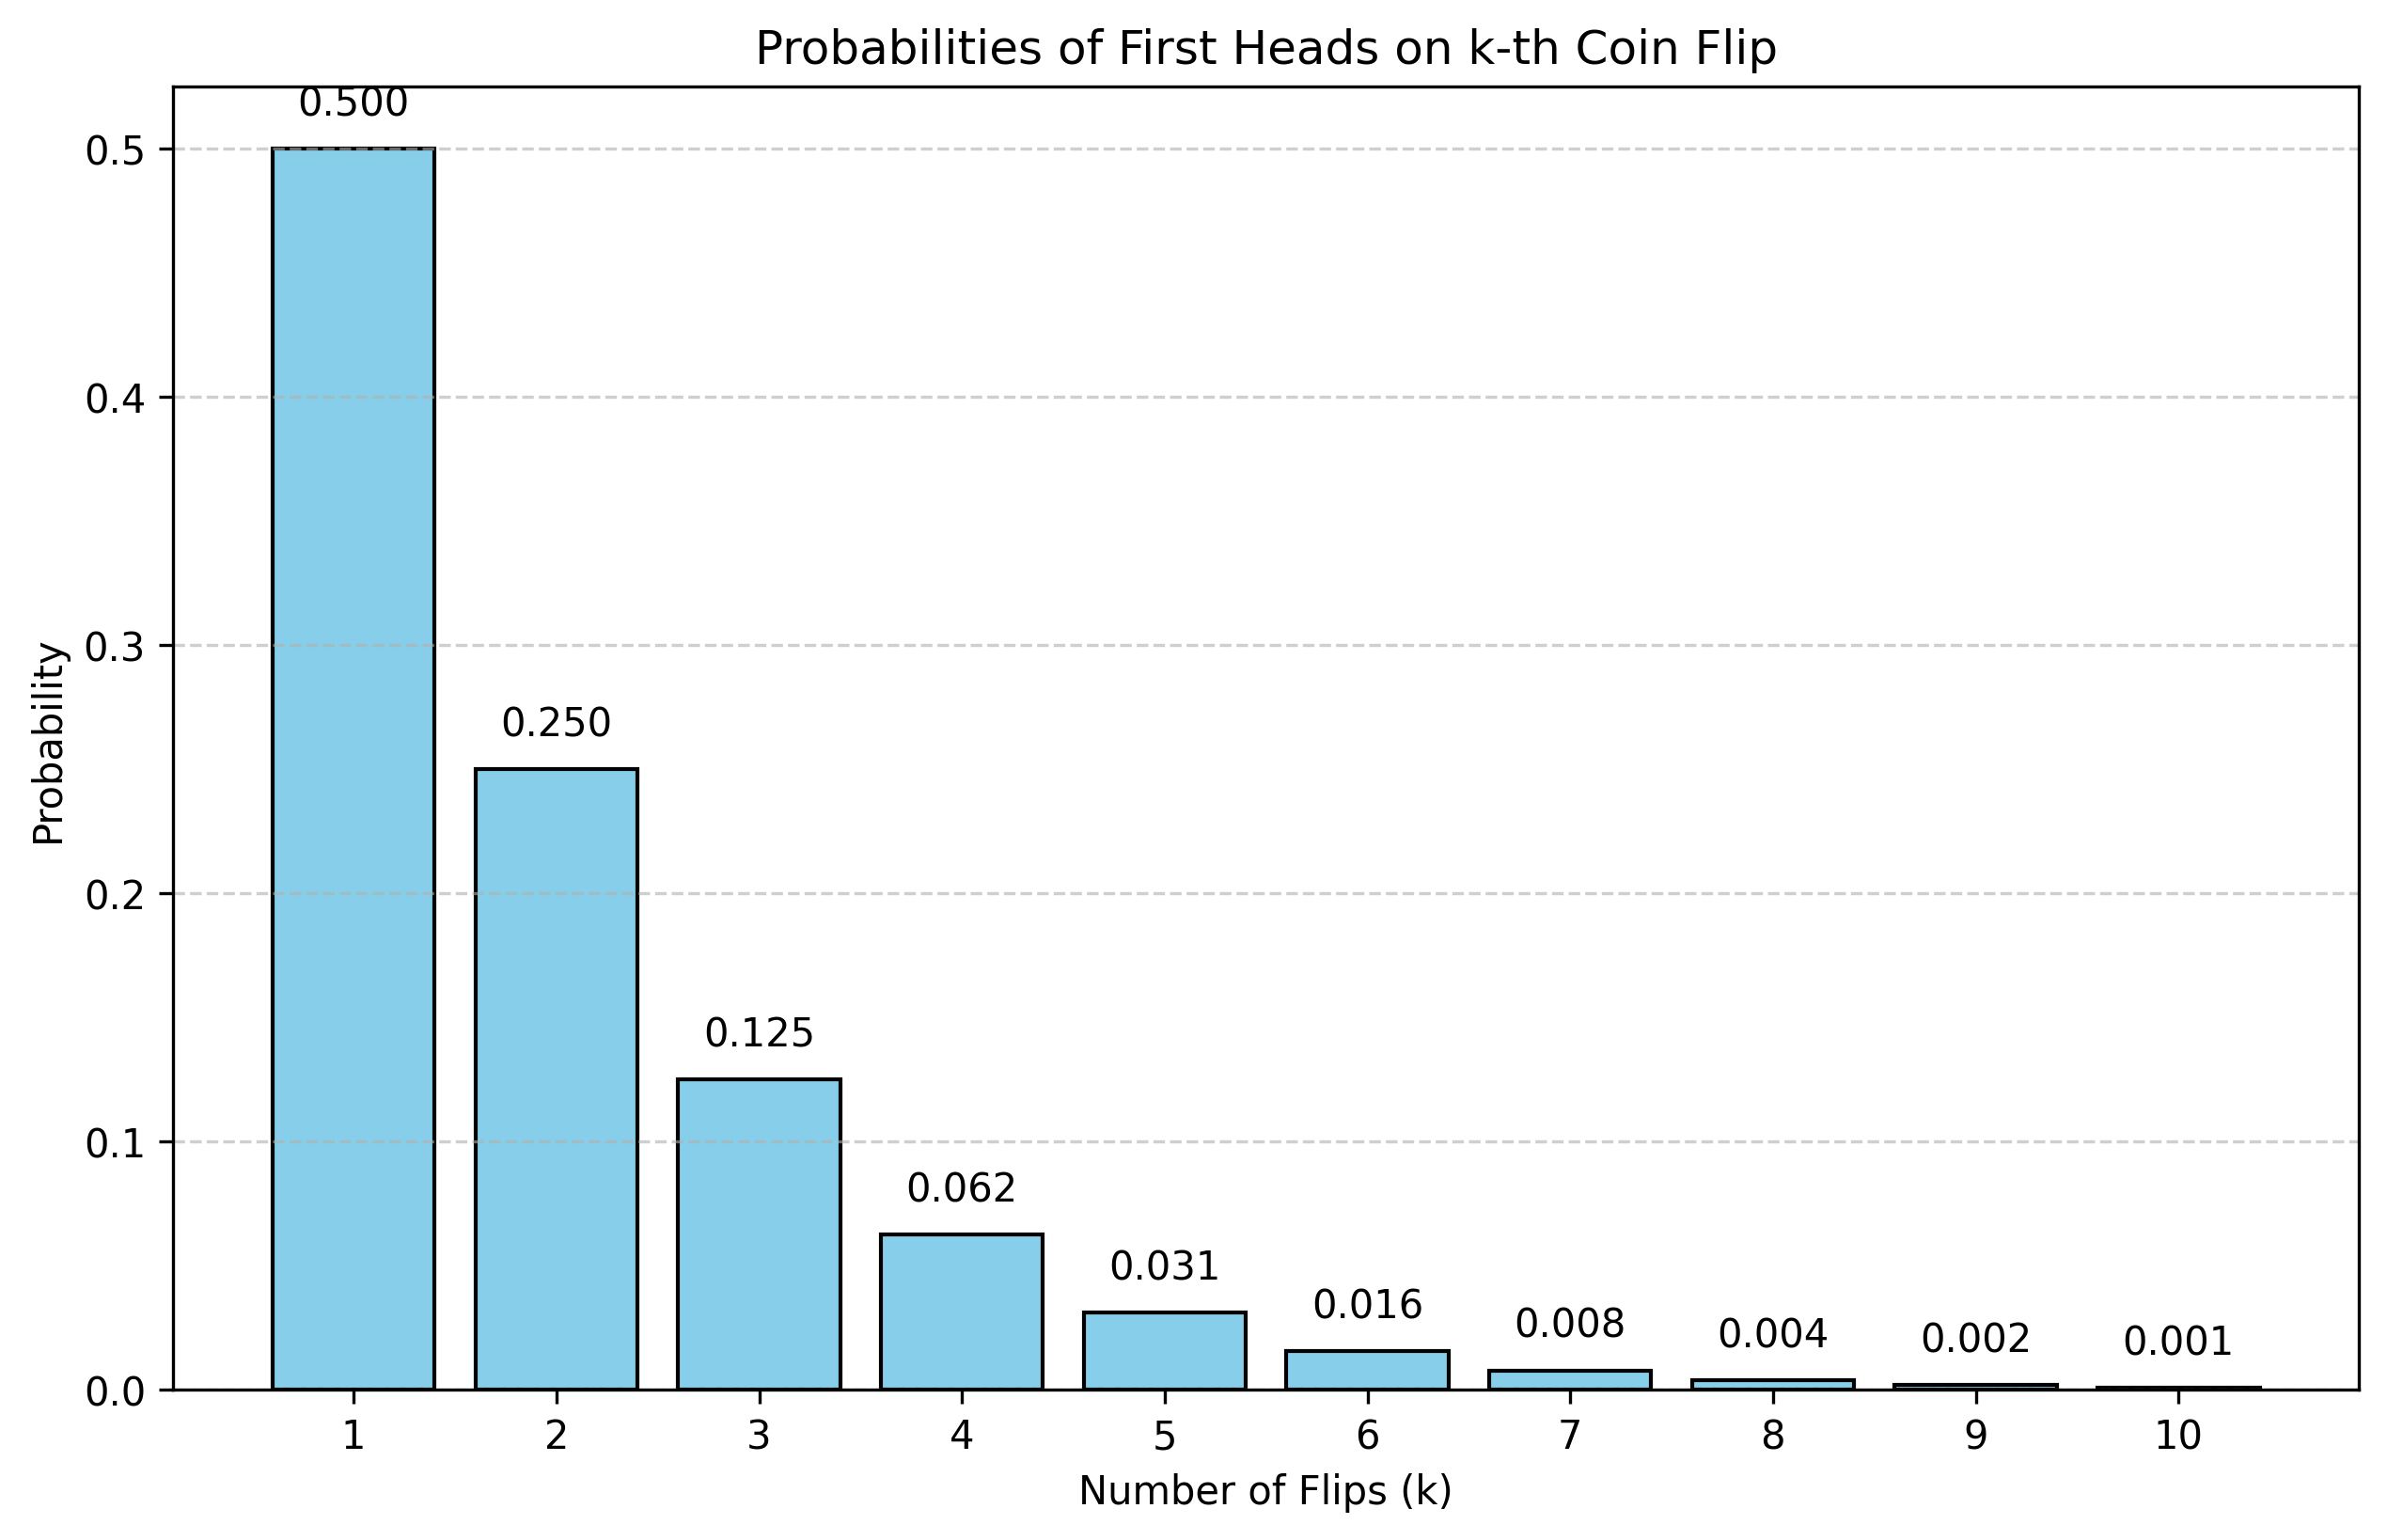
\includegraphics[width=0.8\textwidth]{figure_2_geometric_histogram.png}
  \caption{Histogram of a Geometric Sequence.}
  \label{fig:geom_hist}
\end{figure}

\begin{theorem}[Sum of a Finite Geometric Series \cite{Chan2021}]
The sum of the first $n+1$ terms of a geometric series (starting from $k=0$) with first term $a$ and common ratio $r$ is:
\[
S_n = \sum_{k=0}^{n} a r^k = a + ar + ar^2 + \dots + ar^n = a\frac{1-r^{n+1}}{1-r}, \quad r \neq 1
\]
For the simple case $a=1$: $\sum_{k=0}^{n} r^k = \frac{1-r^{n+1}}{1-r}$.
\end{theorem}

\begin{corollary}[Sum of an Infinite Geometric Series \cite{Chan2021}]
If $0 < |r| < 1$, the sum of an infinite geometric series converges to:
\[
S_{\infty} = \sum_{k=0}^{\infty} a r^k = a + ar + ar^2 + \dots = \frac{a}{1-r}
\]
For the simple case $a=1$: $\sum_{k=0}^{\infty} r^k = \frac{1}{1-r}$.
This works because as $n \rightarrow \infty$, the term $r^{n+1}$ approaches 0.
\end{corollary}

\begin{example}[Note Example]
Compute $\sum_{k=2}^{\infty} \frac{1}{2^k}$.
This series is $\frac{1}{4} + \frac{1}{8} + \frac{1}{16} + \dots$
The first term is $a = 1/4$ and the common ratio is $r = 1/2$. Since $|r|<1$, the series converges.
Using the infinite sum formula:
\[
S_\infty = \frac{a}{1-r} = \frac{1/4}{1 - 1/2} = \frac{1/4}{1/2} = \frac{1}{2}
\]
Alternatively, factor out $1/4$:
\[
= \frac{1}{4} \left(1 + \frac{1}{2} + \frac{1}{4} + \dots\right) = \frac{1}{4} \sum_{k=0}^{\infty} \left(\frac{1}{2}\right)^k = \frac{1}{4} \left( \frac{1}{1 - 1/2} \right) = \frac{1}{4} \cdot 2 = \frac{1}{2}
\]
\end{example}

\begin{corollary}[Derivative of Geometric Series \cite{Chan2021}]
By taking the derivative of the infinite series formula $\sum_{k=0}^{\infty} r^k = \frac{1}{1-r}$ with respect to $r$, we get a useful identity for $0 < |r| < 1$:
\[
\frac{d}{dr} \sum_{k=0}^{\infty} r^k = \frac{d}{dr} \left(\frac{1}{1-r}\right)
\]
\[
\sum_{k=1}^{\infty} k r^{k-1} = 1 + 2r + 3r^2 + \dots = \frac{1}{(1-r)^2}
\]
\end{corollary}

\begin{example}[Note Example]
Compute $\sum_{k=1}^{\infty} k \cdot \frac{2}{3^k}$.
We can manipulate this to match the corollary:
\begin{align*}
    \sum_{k=1}^{\infty} k \cdot \frac{2}{3^k} &= 2 \sum_{k=1}^{\infty} k \cdot \left(\frac{1}{3}\right)^k \\
    &= 2 \cdot \left(\frac{1}{3}\right) \sum_{k=1}^{\infty} k \cdot \left(\frac{1}{3}\right)^{k-1} \\
\end{align*}
Now apply the formula with $r = 1/3$:
\[
= \frac{2}{3} \left( \frac{1}{(1 - 1/3)^2} \right) = \frac{2}{3} \left( \frac{1}{(2/3)^2} \right) = \frac{2}{3} \cdot \frac{1}{4/9} = \frac{2}{3} \cdot \frac{9}{4} = \frac{3}{2}
\]
\end{example}

\subsection{Taylor and Maclaurin Series}
Taylor approximation is a powerful tool for approximating complex, non-linear functions (like $\log(1+x)$) with simpler polynomials. This is especially useful for analysis when $x$ is close to a certain point $a$, e.g., $x \ll 1$ \cite[Sec 1.2]{Chan2021}.

\begin{figure}[h!]
  \centering
  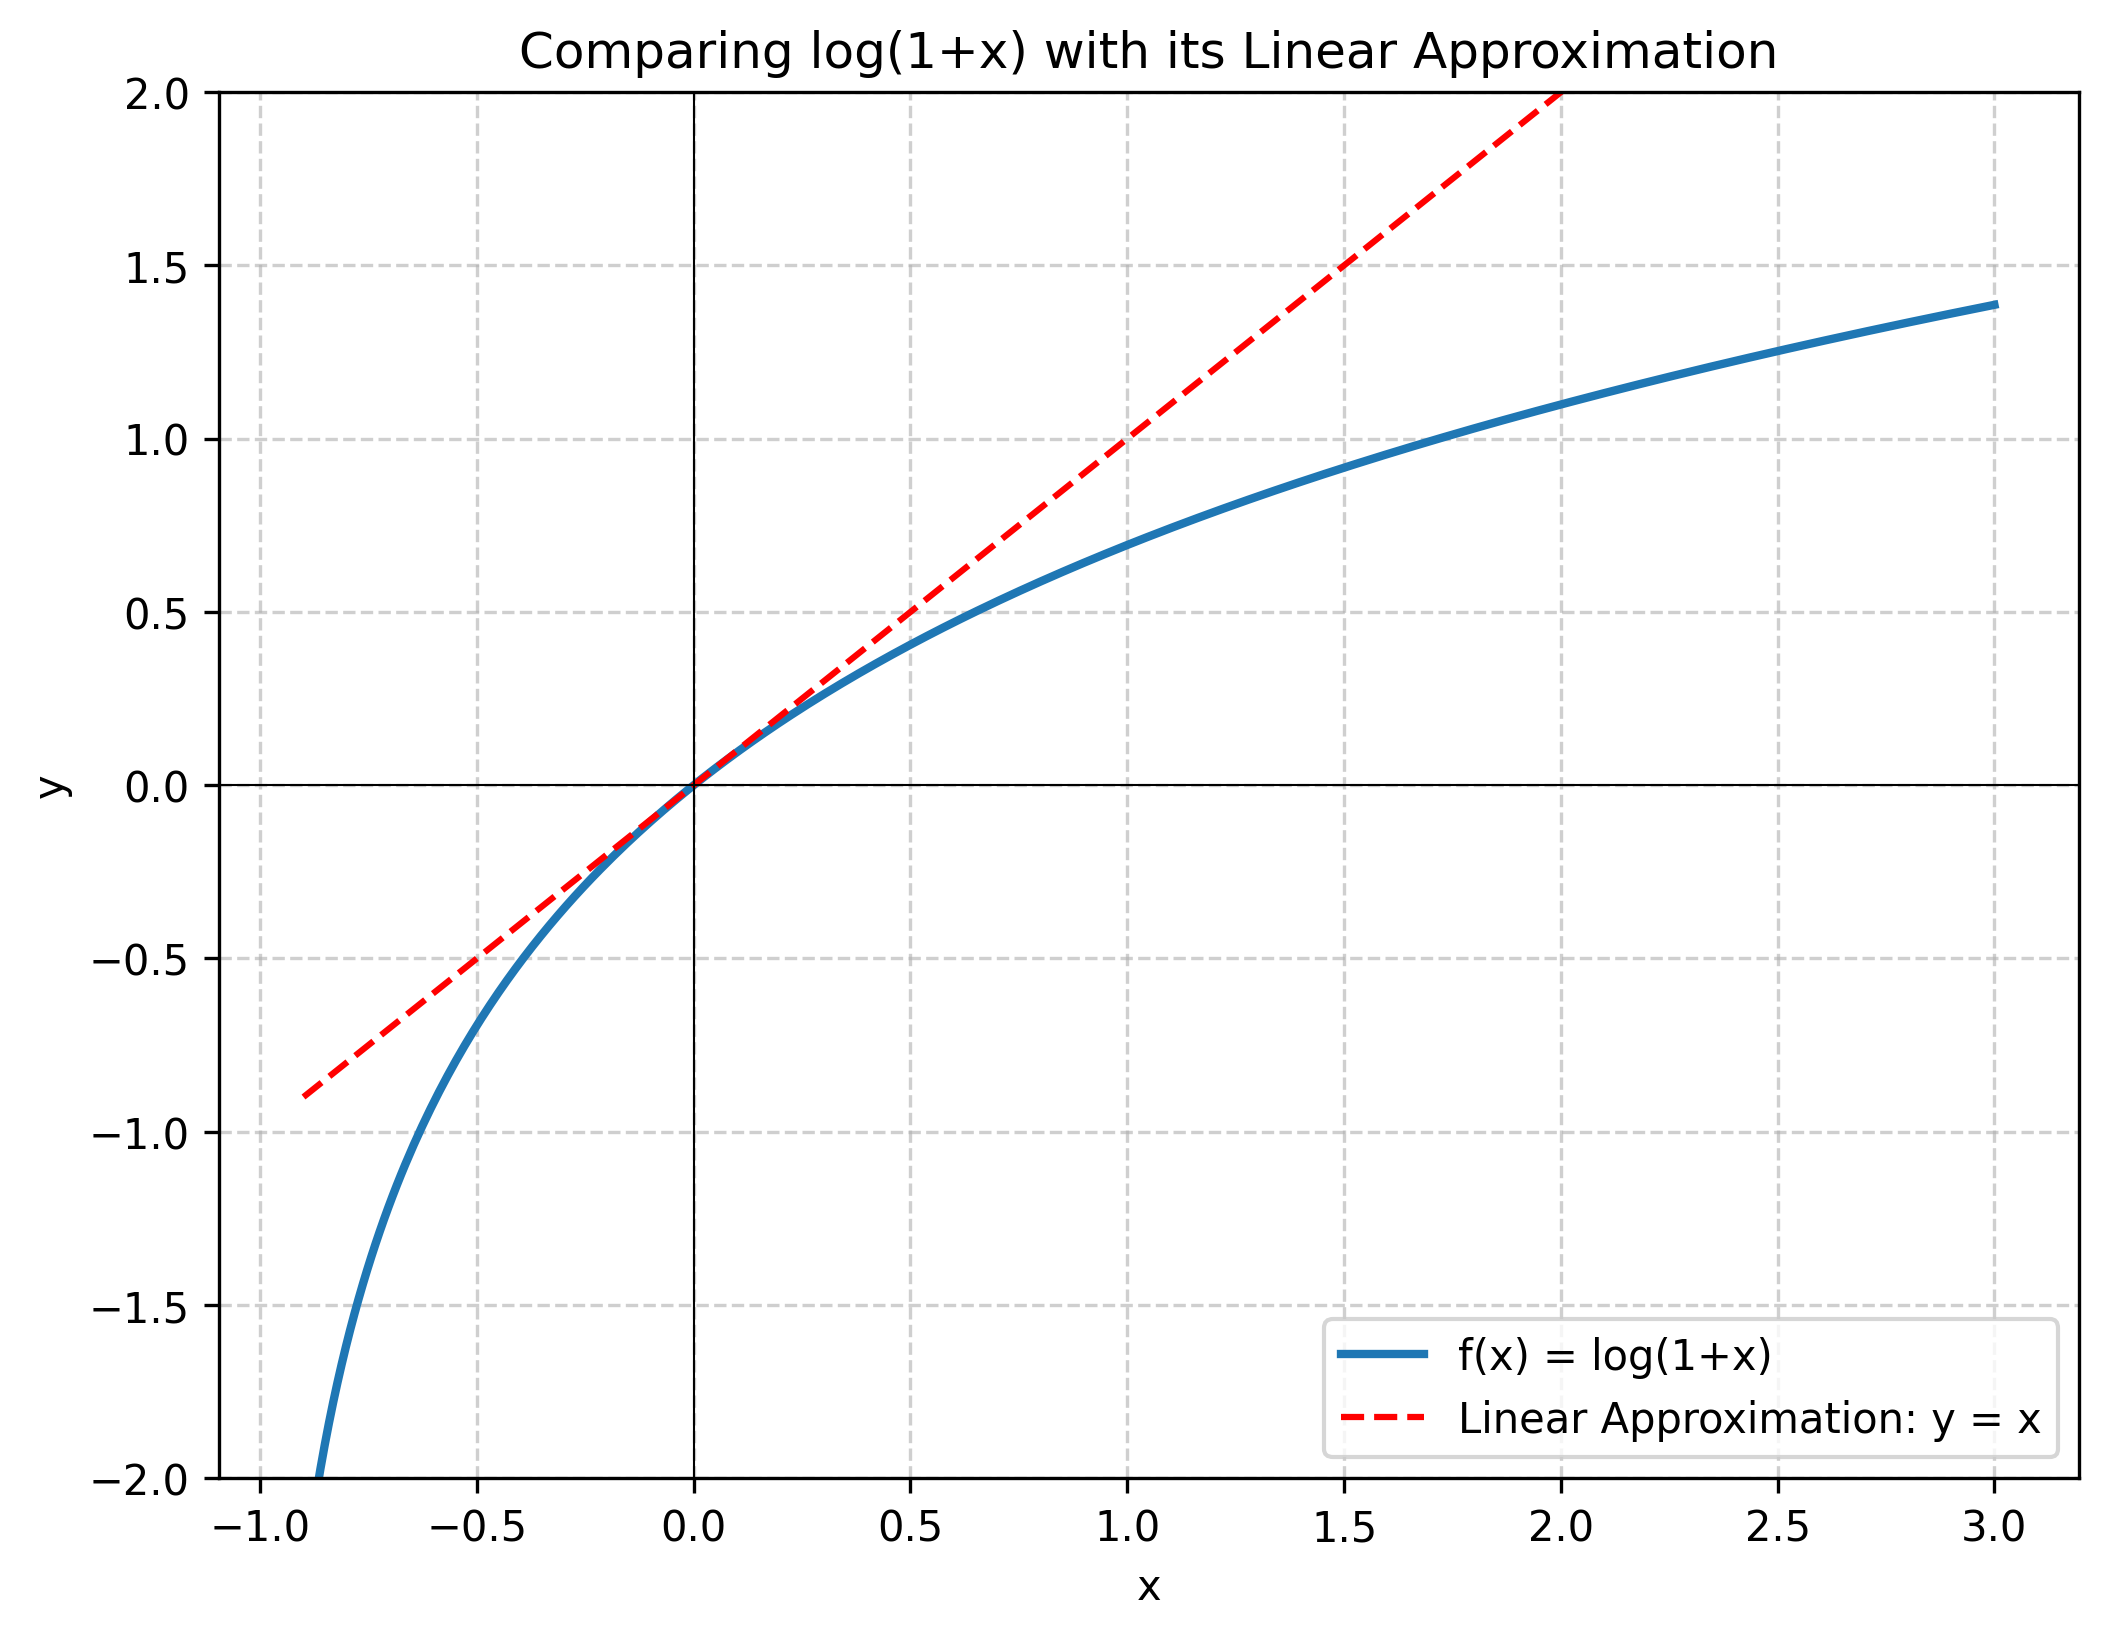
\includegraphics[width=0.8\textwidth]{figure_3_log_approximation.png}
  \caption{Linear approximation of $\log(1+x)$.}
  \label{fig:log_approx}
\end{figure}

\begin{definition}[Taylor Approximation \cite{Chan2021}]
The Taylor approximation of an infinitely differentiable function $f(x)$ at a point $x=a$ is:
\[
f(x) = \sum_{n=0}^{\infty} \frac{f^{(n)}(a)}{n!} (x-a)^n = f(a) + f'(a)(x-a) + \frac{f''(a)}{2!}(x-a)^2 + \dots
\]
When $a=0$, this is called a \textbf{Maclaurin Series}.
\end{definition}

\begin{example}[$f(x) = e^x$ at $a=0$ (Note Example)]
All derivatives $f^{(n)}(x)$ are $e^x$, so $f^{(n)}(0) = e^0 = 1$ for all $n$.
\[
e^x = \sum_{n=0}^{\infty} \frac{1}{n!} (x-0)^n = 1 + x + \frac{x^2}{2!} + \frac{x^3}{3!} + \dots
\]
\end{example}

\begin{example}[$f(x) = \sin x$ at $a=0$ (Note Example)]
The derivatives at $x=0$ follow a pattern: $f(0)=0$, $f'(0)=1$, $f''(0)=0$, $f'''(0)=-1$, etc.
Plugging these into the formula, all the even-powered terms go to zero:
\[
\sin x = 0 + \frac{1}{1!}x + 0 + \frac{-1}{3!}x^3 + 0 + \frac{1}{5!}x^5 + \dots
\]
\[
\sin x = x - \frac{x^3}{3!} + \frac{x^5}{5!} - \frac{x^7}{7!} + \dots
\]
As you include more terms, the approximation becomes more accurate over a wider range.
\end{example}

\begin{figure}[h!]
  \centering
  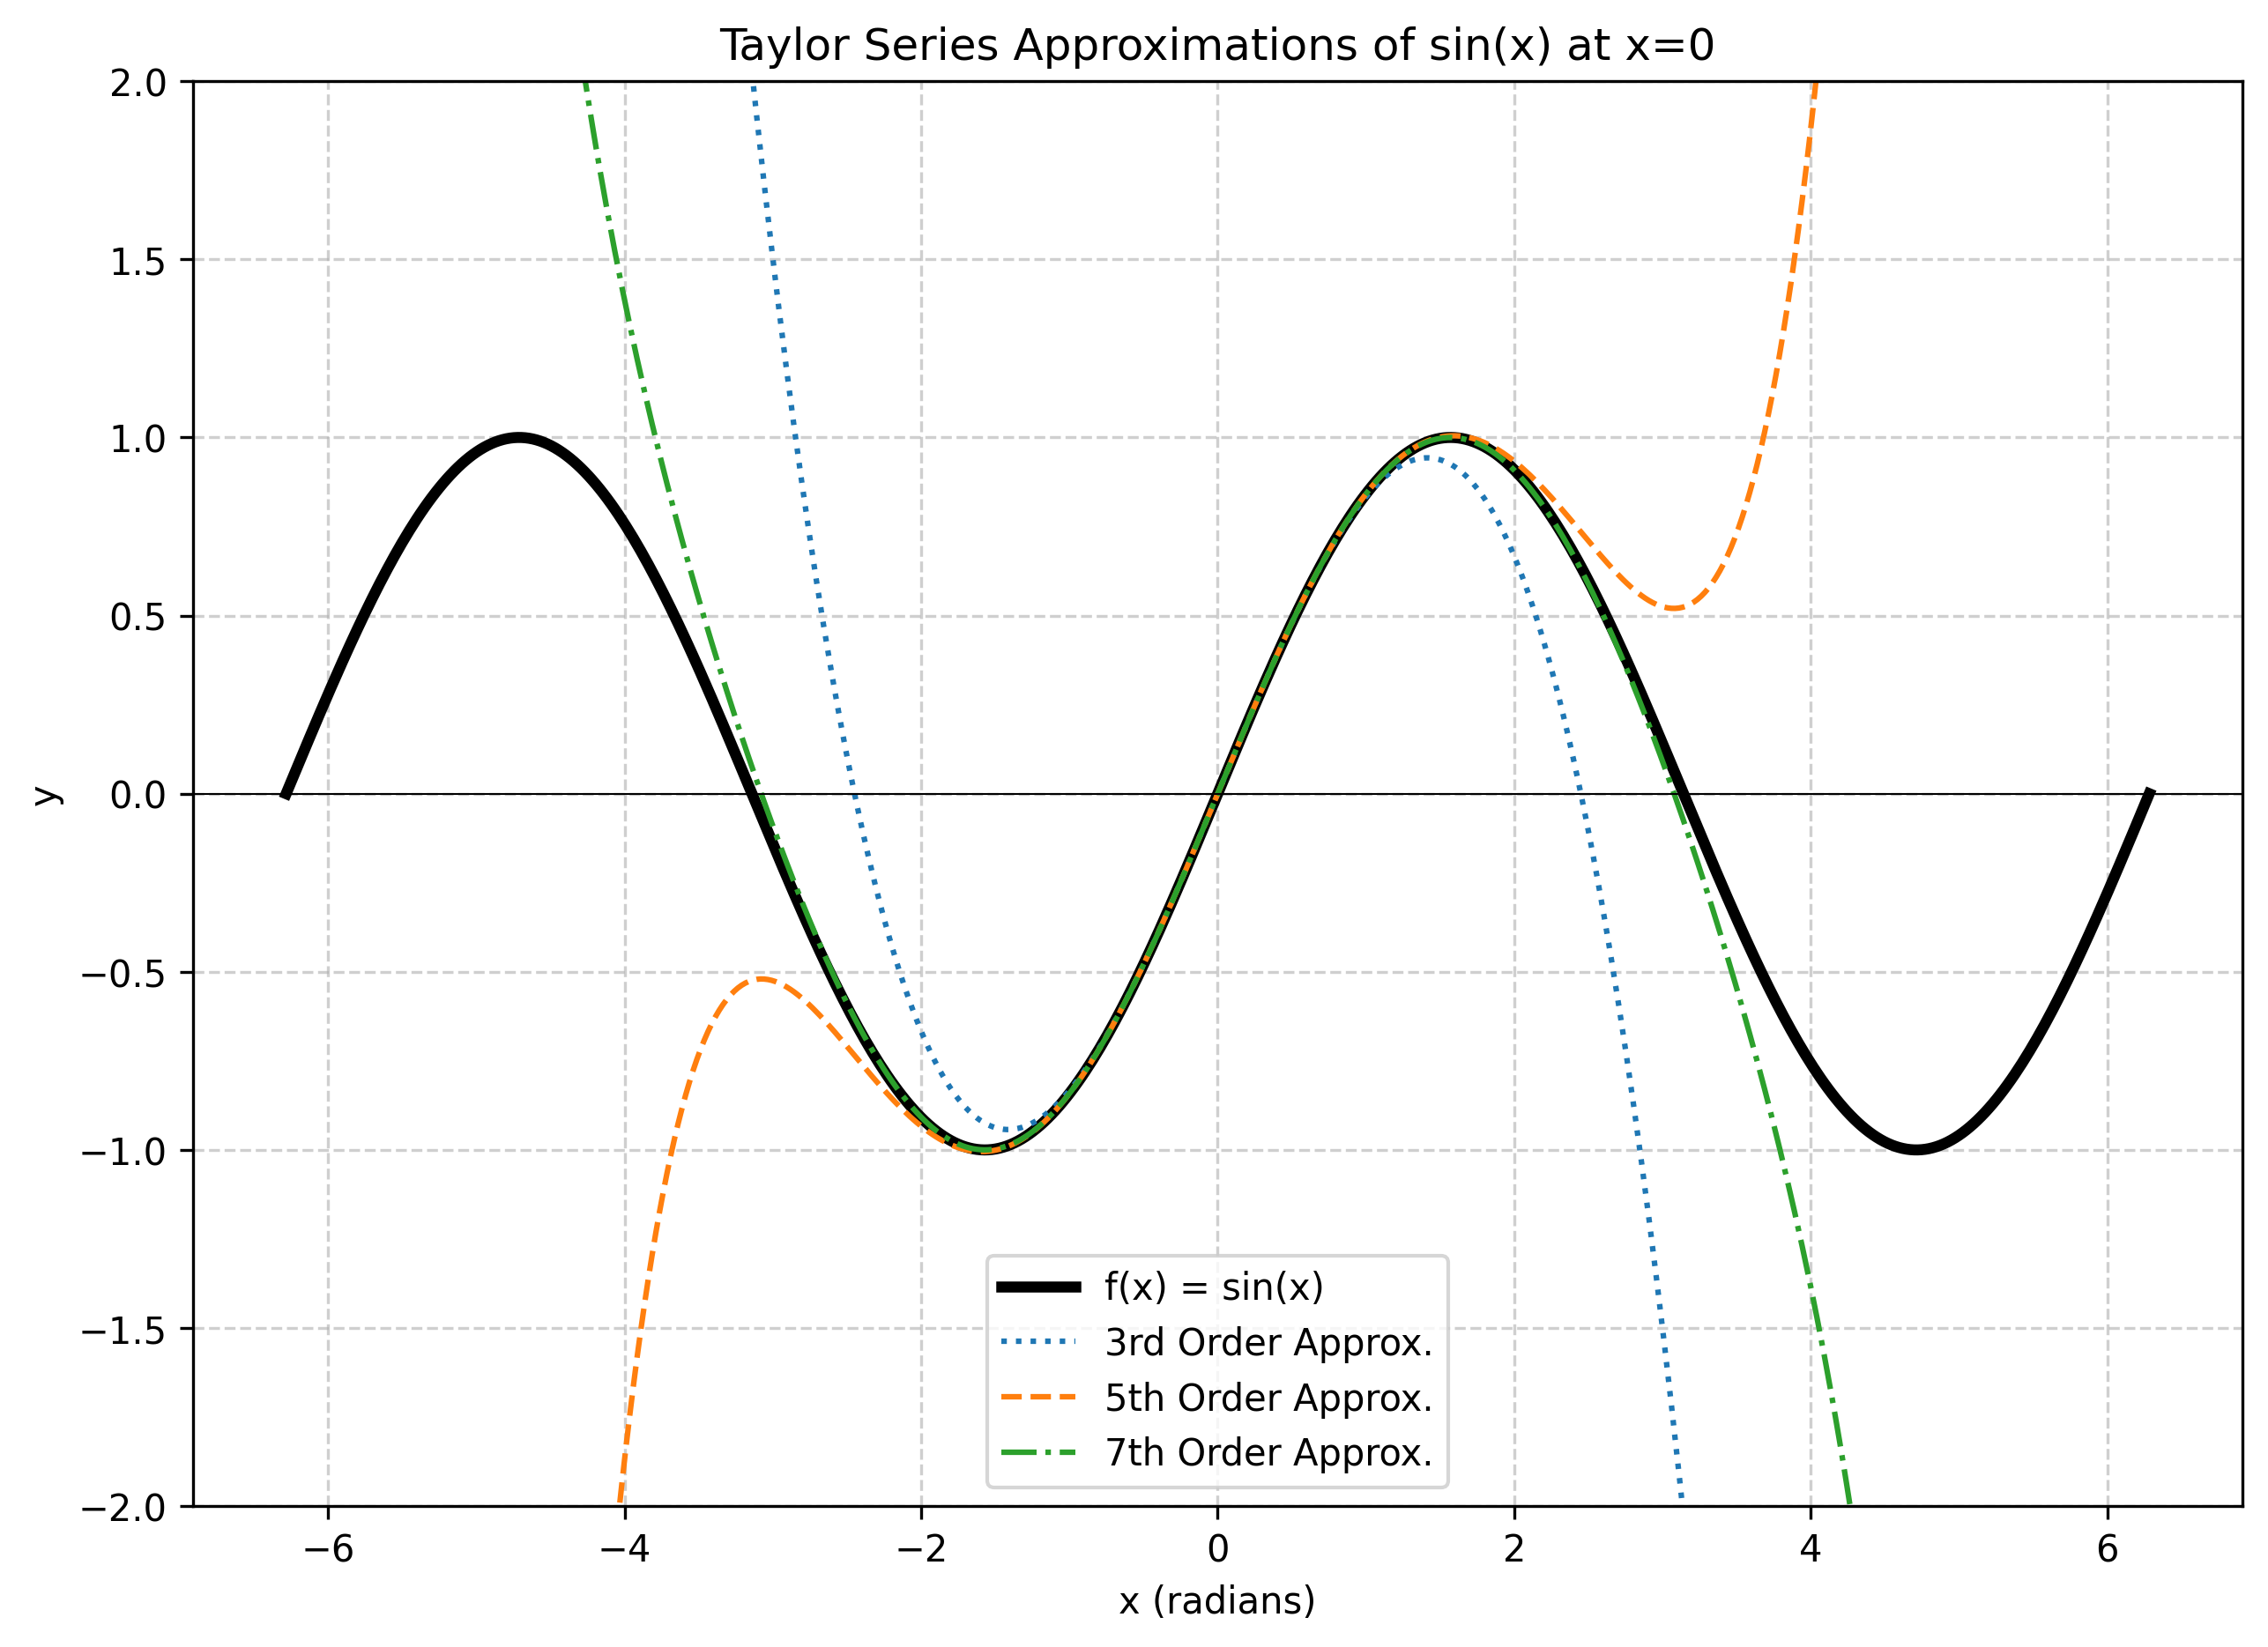
\includegraphics[width=0.8\textwidth]{figure_4_sin_taylor.png}
  \caption{Taylor approximations of $\sin(x)$.}
  \label{fig:sin_approx}
\end{figure}

\newpage
\section{Combinatorics}
Combinatorics is the field of mathematics concerned with counting configurations of discrete events.

\begin{example}[Motivating Example: Birthday Paradox \cite{Chan2021}]
In a room of $k$ people, what is the probability that at least one pair shares a birthday?
It's easier to calculate the complement: the probability that \textit{no one} shares a birthday (assuming 365 days).
\begin{itemize}
    \item Person 1: $\frac{365}{365}$ (can have any birthday)
    \item Person 2: $\frac{364}{365}$ (must be different from person 1)
    \item Person 3: $\frac{363}{365}$ (must be different from 1 and 2)
    \item \dots
    \item Person k: $\frac{365 - k + 1}{365}$
\end{itemize}
The probability of all $k$ people having different birthdays is:
\[
P(\text{all different}) = \frac{365 \times 364 \times \dots \times (365-k+1)}{365^k} = \frac{365!}{(365-k)!} \times \frac{1}{365^{k}}
\]
For $k=50$ people, $P(\text{all different}) \approx 0.03$.
So, the probability of at least one match is $P(\text{match}) = 1 - 0.03 = 0.97$, or 97\%!
\end{example}

\subsection{Permutation}
A permutation is an \textbf{ordered} arrangement of $k$ items selected from a set of $n$ distinct items without replacement.

\begin{theorem}[Number of Permutations \cite{Chan2021}]
The number of ways to choose $k$ ordered items from $n$ is:
\[
P(n, k) = n(n-1)(n-2)\dots(n-k+1) = \frac{n!}{(n-k)!}
\]
\end{theorem}

\begin{example}[Note Example]
How many ways to award 1st, 2nd, and 3rd prize (ordered) from 100 contestants?
\[
P(100, 3) = \frac{100!}{(100-3)!} = \frac{100!}{97!} = 100 \times 99 \times 98 = 970,200
\]
\end{example}

\begin{example}[String Permutations (Note Example)]
How many permutations of the letters \textbf{ABCDEFG} contain:
\begin{enumerate}
    \item[a)] \textbf{the string BCD?}
    Treat (BCD) as a single block. We are permuting (BCD), A, E, F, G.
    These are 5 distinct items. So, the total permutations is $5! = 120$.
    
    \item[b)] \textbf{the strings BA and GF?}
    Treat (BA) and (GF) as single blocks. We are permuting (BA), (GF), C, D, E.
    These are 5 distinct items. So, the total permutations is $5! = 120$.
    
    \item[c)] \textbf{the strings ABC and CDE?}
    This implies the string must be (ABCDE). We are permuting (ABCDE), F, G.
    These are 3 distinct items. So, the total permutations is $3! = 6$.

    \item[d)] \textbf{the strings CBA and BED?}
    This is impossible, as the letter 'B' must be in two different positions simultaneously. The number of permutations is 0.
\end{enumerate}
\end{example}

\subsection{Combination}
A combination is an \textbf{unordered} selection of $k$ items from a set of $n$ distinct items without replacement. The order of selection does not matter.

\begin{theorem}[Number of Combinations \cite{Chan2021}]
This is also called "n choose k" or the binomial coefficient.
\[
C(n, k) = \binom{n}{k} = \frac{P(n, k)}{k!} = \frac{n!}{k!(n-k)!}
\]
We divide the number of permutations by $k!$ because there are $k!$ ways to order the $k$ chosen items, and in a combination, all those orderings are counted as one.
\end{theorem}

\begin{example}[Note Example]
How many 5-card poker hands (unordered) can be dealt from a standard 52-card deck?
\[
C(52, 5) = \binom{52}{5} = \frac{52!}{5!(52-5)!} = \frac{52!}{5!47!} = 2,598,960
\]
\end{example}

\begin{example}[Note Example]
How many ways to select a 6-person crew (unordered) from 30 astronauts?
\[
C(30, 6) = \binom{30}{6} = \frac{30!}{6!(30-6)!} = \frac{30!}{6!24!} = 593,775
\]
\end{example}

\subsection{The Binomial Theorem}
The binomial theorem uses combinations (binomial coefficients) to expand a binomial raised to a power.

\begin{theorem}[Binomial Theorem \cite{Chan2021}]
For any real numbers $a$ and $b$ and integer $n \ge 0$:
\[
(a+b)^n = \sum_{k=0}^{n} \binom{n}{k} a^{n-k} b^k
\]
\end{theorem}

\begin{example}[Note Example]
Expand $(x+y)^4$.
\begin{align*}
(x+y)^4 &= \binom{4}{0}x^4y^0 + \binom{4}{1}x^3y^1 + \binom{4}{2}x^2y^2 + \binom{4}{3}x^1y^3 + \binom{4}{4}x^0y^4 \\
&= 1x^4 + 4x^3y + 6x^2y^2 + 4xy^3 + 1y^4
\end{align*}
\end{example}

\begin{example}[Note Example]
What is the coefficient of $x^{12}y^{13}$ in the expansion of $(x+y)^{25}$?
The term with $y^{13}$ corresponds to $k=13$.
The term is $\binom{25}{13} x^{25-13} y^{13} = \binom{25}{13} x^{12} y^{13}$.
The coefficient is $\binom{25}{13} = \frac{25!}{13!(25-13)!} = \frac{25!}{13!12!}$.
\end{example}

\begin{example}[Note Example]
What is the coefficient of $x^{12}y^{13}$ in the expansion of $(2x-3y)^{25}$?
Let $a = 2x$ and $b = -3y$. We need the term with $b^{13}$, which corresponds to $k=13$.
The term is $\binom{25}{13} a^{25-13} b^{13} = \binom{25}{13} (2x)^{12} (-3y)^{13}$.
\[
= \binom{25}{13} 2^{12} x^{12} (-3)^{13} y^{13} = \binom{25}{13} 2^{12} (-1)^{13} 3^{13} x^{12} y^{13}
\]
The coefficient is $-\binom{25}{13} 2^{12} 3^{13} = -\frac{25!}{12! 13!} 2^{12} 3^{13}$.
\end{example}

\begin{example}[Binomial Identities (Note Example)]
By cleverly choosing $a$ and $b$, we can prove identities:
\begin{enumerate}
    \item \textbf{Let $a=1, b=1$}: $(1+1)^n = \sum_{k=0}^{n} \binom{n}{k} (1)^{n-k} (1)^k \implies \mathbf{2^n = \sum_{k=0}^{n} \binom{n}{k}}$
    \item \textbf{Let $a=1, b=-1$}: $(1-1)^n = \sum_{k=0}^{n} \binom{n}{k} (1)^{n-k} (-1)^k \implies \mathbf{0 = \sum_{k=0}^{n} (-1)^k \binom{n}{k}}$
    \item \textbf{Let $a=1, b=2$}: $(1+2)^n = \sum_{k=0}^{n} \binom{n}{k} (1)^{n-k} (2)^k \implies \mathbf{3^n = \sum_{k=0}^{n} 2^k \binom{n}{k}}$
\end{enumerate}
\end{example}

\subsection{Pascal's Identity}
This identity shows how the coefficients in one row of Pascal's triangle are formed from the row above it.

\begin{theorem}[Pascal's Identity \cite{Chan2021}]
Let n and k be positive integers with $1 \le k \le n$. Then:
\[
\binom{n+1}{k} = \binom{n}{k-1} + \binom{n}{k}
\]
\end{theorem}

\begin{figure}[h!]
  \centering
  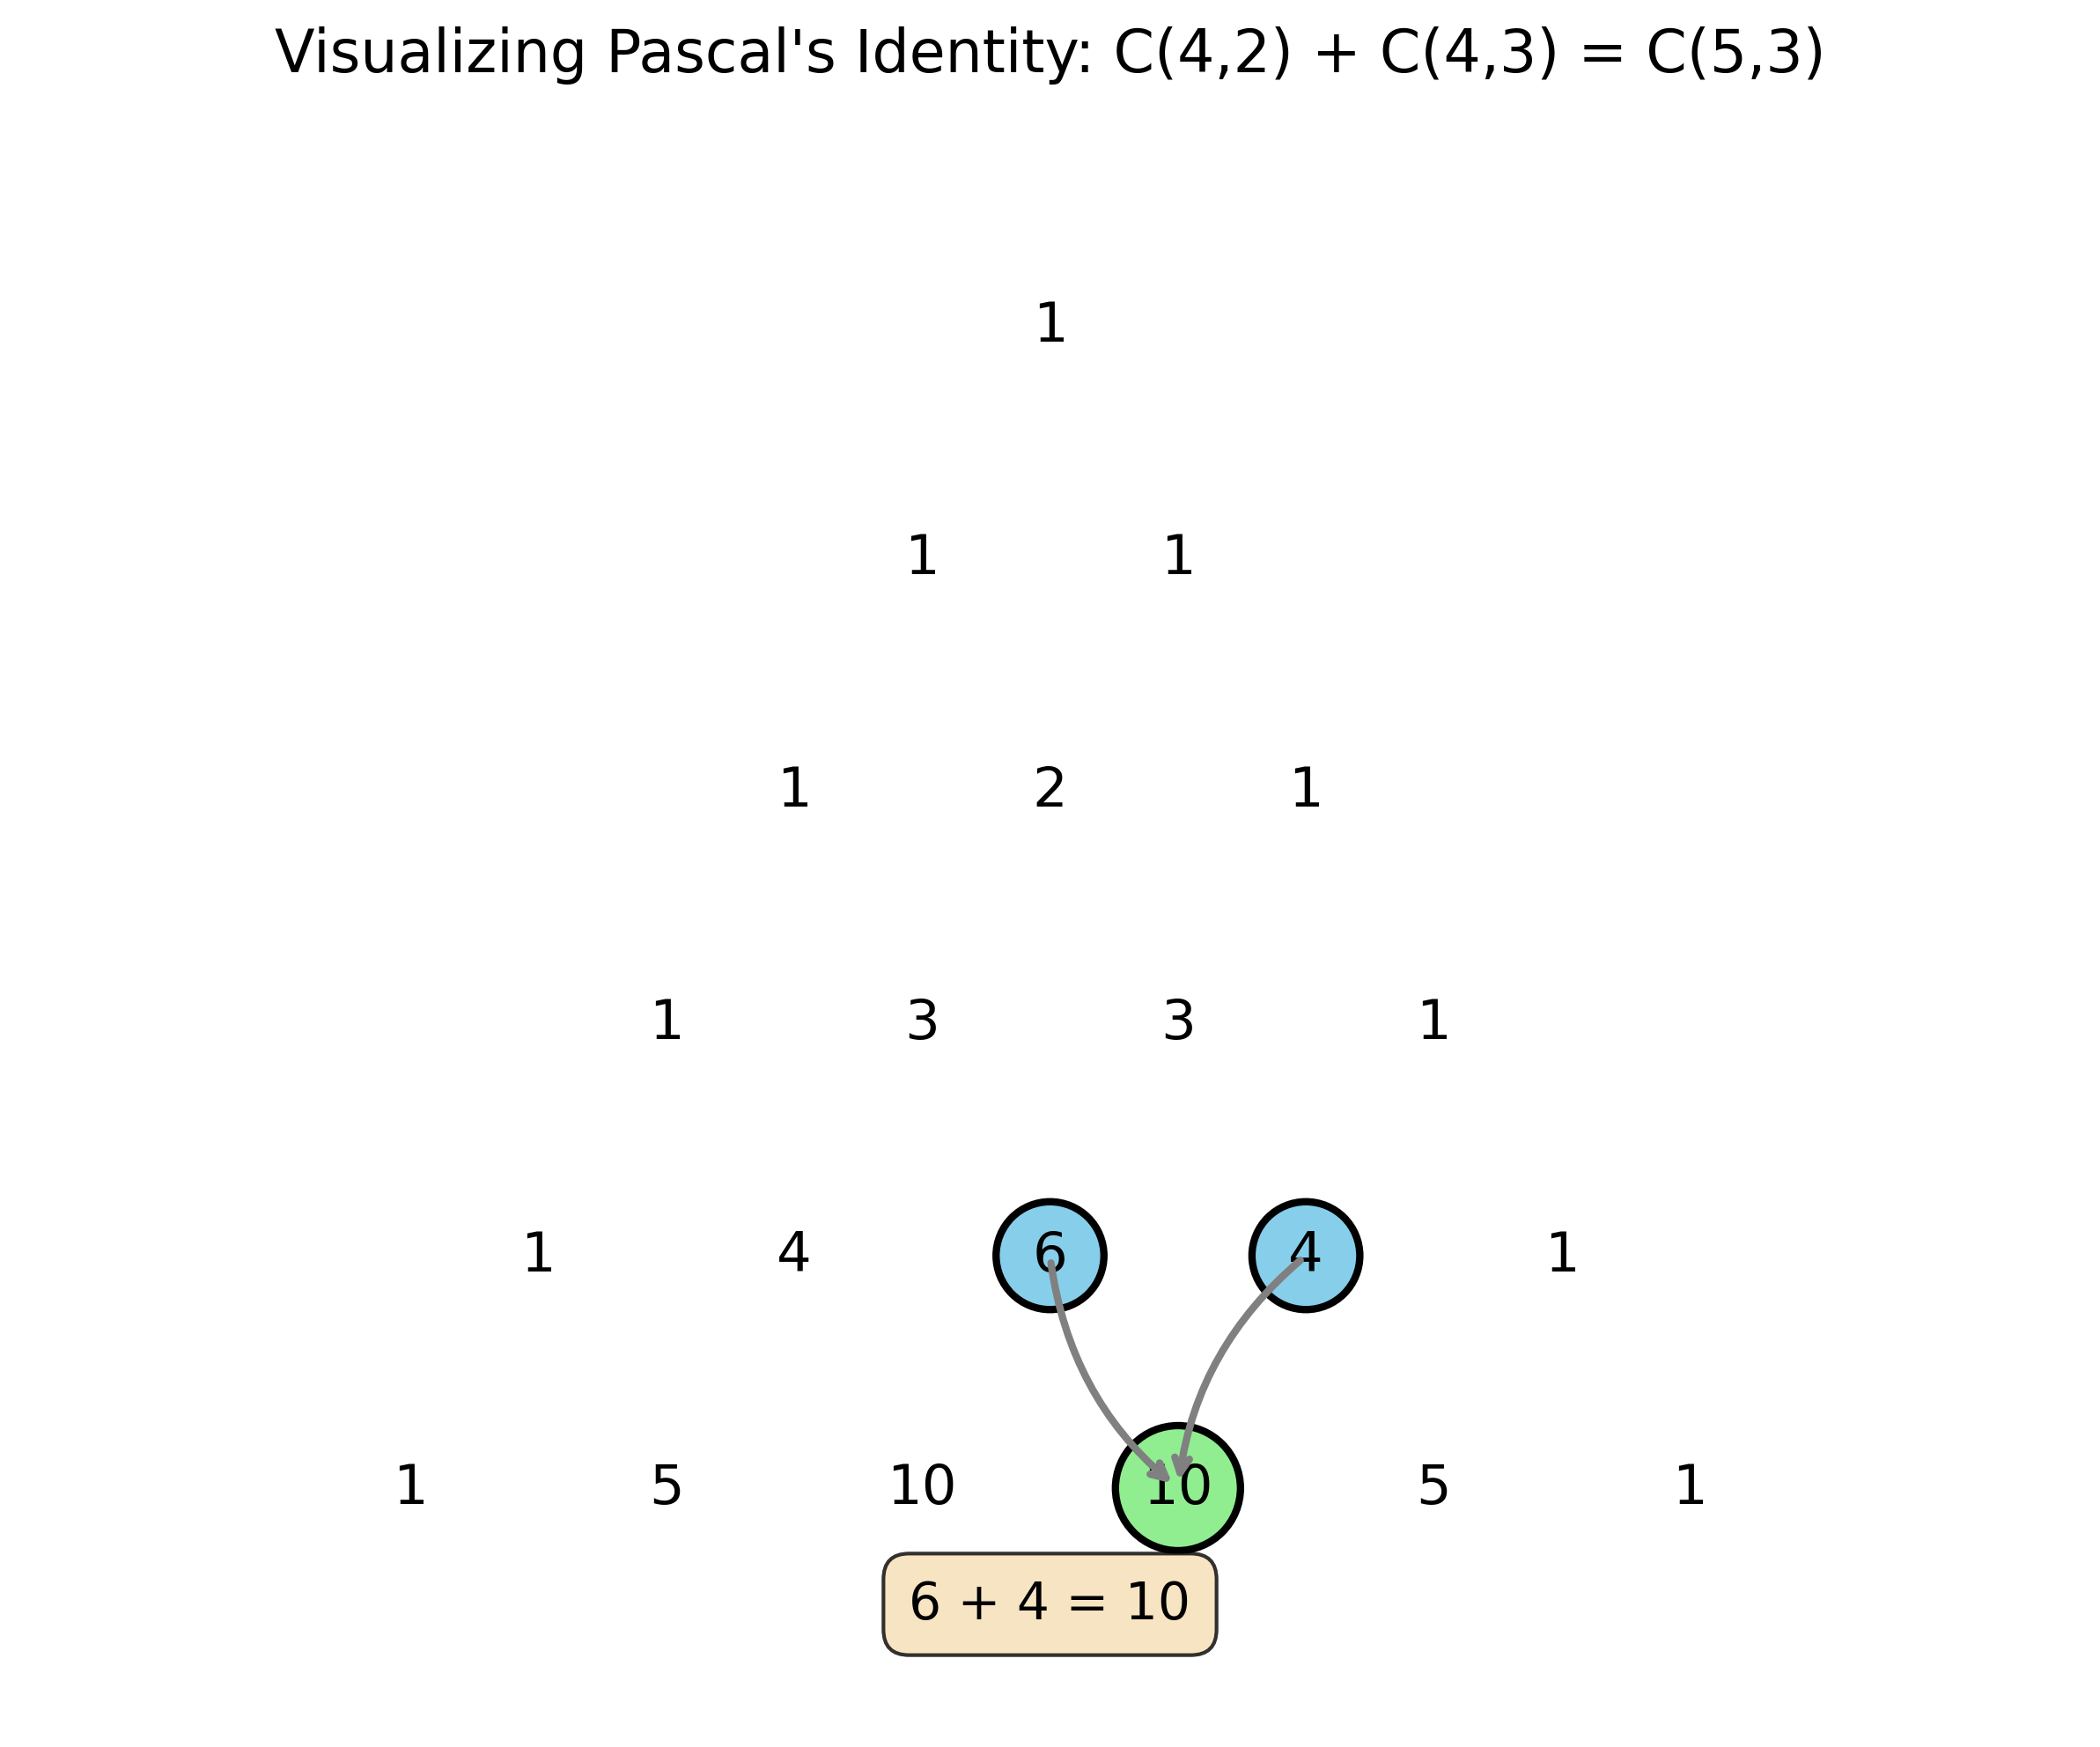
\includegraphics[width=0.8\textwidth]{figure_5_pascals_identity.png}
  \caption{Pascal's Identity in the triangle.}
  \label{fig:pascal}
\end{figure}

\newpage
\section{Integration Techniques}
Integration is a core concept in calculus, often used to find the area under probability density functions to calculate probabilities.

\subsection{Integration by Substitution}
Used when an integrand contains a function and its derivative.
\begin{example}[Note Example]
$\int 2x \cos(x^2) dx$.
Let $u = x^2$, so $du = 2x dx$.
\[
\int \cos(u) du = \sin(u) + C = \sin(x^2) + C
\]
\end{example}

\begin{example}[Note Example]
$\int x^3 \sqrt{1-x^2} dx$.
Let $u = 1-x^2$. Then $du = -2x dx \Rightarrow x dx = -du/2$. Also, $x^2 = 1-u$.
Rewrite the integral:
\begin{align*}
    \int x^3 \sqrt{1-x^2} dx &= \int x^2 \sqrt{1-x^2} (x dx) \\
    &= \int (1-u) \sqrt{u} \left(-\frac{du}{2}\right) \\
    &= -\frac{1}{2} \int (u^{1/2} - u^{3/2}) du \\
    &= -\frac{1}{2} \left[ \frac{u^{3/2}}{3/2} - \frac{u^{5/2}}{5/2} \right] + C \\
    &= -\frac{1}{3}u^{3/2} + \frac{1}{5}u^{5/2} + C \\
    &= \frac{1}{5}(1-x^2)^{5/2} - \frac{1}{3}(1-x^2)^{3/2} + C
\end{align*}
\end{example}

\subsection{Method of Partial Fractions}
Used to integrate rational functions (a polynomial divided by another).
\begin{example}[Note Example]
Decompose $\frac{5x-3}{(x+1)(x-3)}$.
\[
\frac{5x-3}{(x+1)(x-3)} = \frac{A}{x+1} + \frac{B}{x-3}
\]
Clear the denominator: $5x-3 = A(x-3) + B(x+1)$.
\begin{itemize}
    \item Let $x=3$: $5(3)-3 = A(0) + B(3+1) \Rightarrow 12 = 4B \Rightarrow B=3$
    \item Let $x=-1$: $5(-1)-3 = A(-1-3) + B(0) \Rightarrow -8 = -4A \Rightarrow A=2$
\end{itemize}
So,
\[
\frac{5x-3}{(x+1)(x-3)} = \frac{2}{x+1} + \frac{3}{x-3}
\]
\end{example}

\begin{example}[Partial Fractions with Repeated/Irreducible Roots (Note Example)]
Decompose $\frac{-2x+4}{(x^2+1)(x-1)^2}$.
The form includes a linear term for the irreducible quadratic ($x^2+1$) and terms for the repeated root ($x-1$).
\[
\frac{-2x+4}{(x^2+1)(x-1)^2} = \frac{Ax+B}{x^2+1} + \frac{C}{x-1} + \frac{D}{(x-1)^2}
\]
Clear the denominator:
\begin{align*}
-2x+4 &= (Ax+B)(x-1)^2 + C(x^2+1)(x-1) + D(x^2+1) \\
&= (Ax+B)(x^2-2x+1) + C(x^3-x^2+x-1) + D(x^2+1) \\
&= (Ax^3 - 2Ax^2 + Ax + Bx^2 - 2Bx + B) + (Cx^3 - Cx^2 + Cx - C) + (Dx^2 + D)
\end{align*}
Group by powers of $x$:
\[
-2x+4 = (A+C)x^3 + (-2A+B-C+D)x^2 + (A-2B+C)x + (B-C+D)
\]
Equate coefficients:
\begin{enumerate}
    \item $x^3$: $A+C = 0 \implies C = -A$
    \item $x^0$: $B-C+D = 4$
    \item $x^1$: $A-2B+C = -2 \implies A-2B-A = -2 \implies -2B = -2 \implies \mathbf{B=1}$
    \item $x^2$: $-2A+B-C+D = 0$. Substitute $B=1$ and $B-C+D=4$ into this: \\ $-2A+(B-C+D) = 0 \implies -2A + 4 = 0 \implies \mathbf{A=2}$
\end{enumerate}
From the other equations:
\begin{itemize}
    \item $C = -A \implies \mathbf{C=-2}$
    \item $B-C+D = 4 \implies 1 - (-2) + D = 4 \implies 3 + D = 4 \implies \mathbf{D=1}$
\end{itemize}
So,
\[
\frac{-2x+4}{(x^2+1)(x-1)^2} = \frac{2x+1}{x^2+1} - \frac{2}{x-1} + \frac{1}{(x-1)^2}
\]
\end{example}

\begin{example}[Integration with Partial Fractions (Note Example)]
$\int \frac{x+4}{x^3+3x^2-10x} dx$.
\begin{enumerate}
    \item \textbf{Factor denominator:} $x(x^2+3x-10) = x(x+5)(x-2)$.
    \item \textbf{Set up fractions:}
    \[
    \frac{x+4}{x(x+5)(x-2)} = \frac{A}{x} + \frac{B}{x+5} + \frac{C}{x-2}
    \]
    \item \textbf{Solve for A, B, C (Cover-up Method):}
    \begin{itemize}
        \item For $A$ (cover $x$, plug in $x=0$): $A = \frac{0+4}{(0+5)(0-2)} = \frac{4}{-10} = -\frac{2}{5}$
        \item For $B$ (cover $x+5$, plug in $x=-5$): $B = \frac{-5+4}{(-5)(-5-2)} = \frac{-1}{(-5)(-7)} = -\frac{1}{35}$
        \item For $C$ (cover $x-2$, plug in $x=2$): $C = \frac{2+4}{(2)(2+5)} = \frac{6}{14} = \frac{3}{7}$
    \end{itemize}
    \item \textbf{Integrate:}
    \[
    \int \left( -\frac{2}{5x} - \frac{1}{35(x+5)} + \frac{3}{7(x-2)} \right) dx
    \]
    \[
    = -\frac{2}{5}\ln|x| - \frac{1}{35}\ln|x+5| + \frac{3}{7}\ln|x-2| + C
    \]
\end{enumerate}
\end{example}

\subsection{Odd and Even Functions}
This is a simplification for integrals over symmetric intervals, like $\int_{-a}^{a} f(x) dx$ \cite[Sec 1.3.1]{Chan2021}.
\begin{itemize}
    \item An \textbf{even function} is symmetric about the y-axis, where $f(x) = f(-x)$.
    \[
    \int_{-a}^{a} f(x) dx = 2 \int_{0}^{a} f(x) dx
    \]
    \item An \textbf{odd function} is anti-symmetric, where $f(x) = -f(-x)$.
    \[
    \int_{-a}^{a} f(x) dx = 0
    \]
\end{itemize}
\begin{example}[Odd Function]
$f(x) = x e^{-x^2/2}$ is odd, since $f(-x) = (-x)e^{-(-x)^2/2} = -xe^{-x^2/2} = -f(x)$.
Therefore, $\int_{-5}^{5} x e^{-x^2/2} dx = 0$.
\end{example}

\begin{figure}[h!]
  \centering
  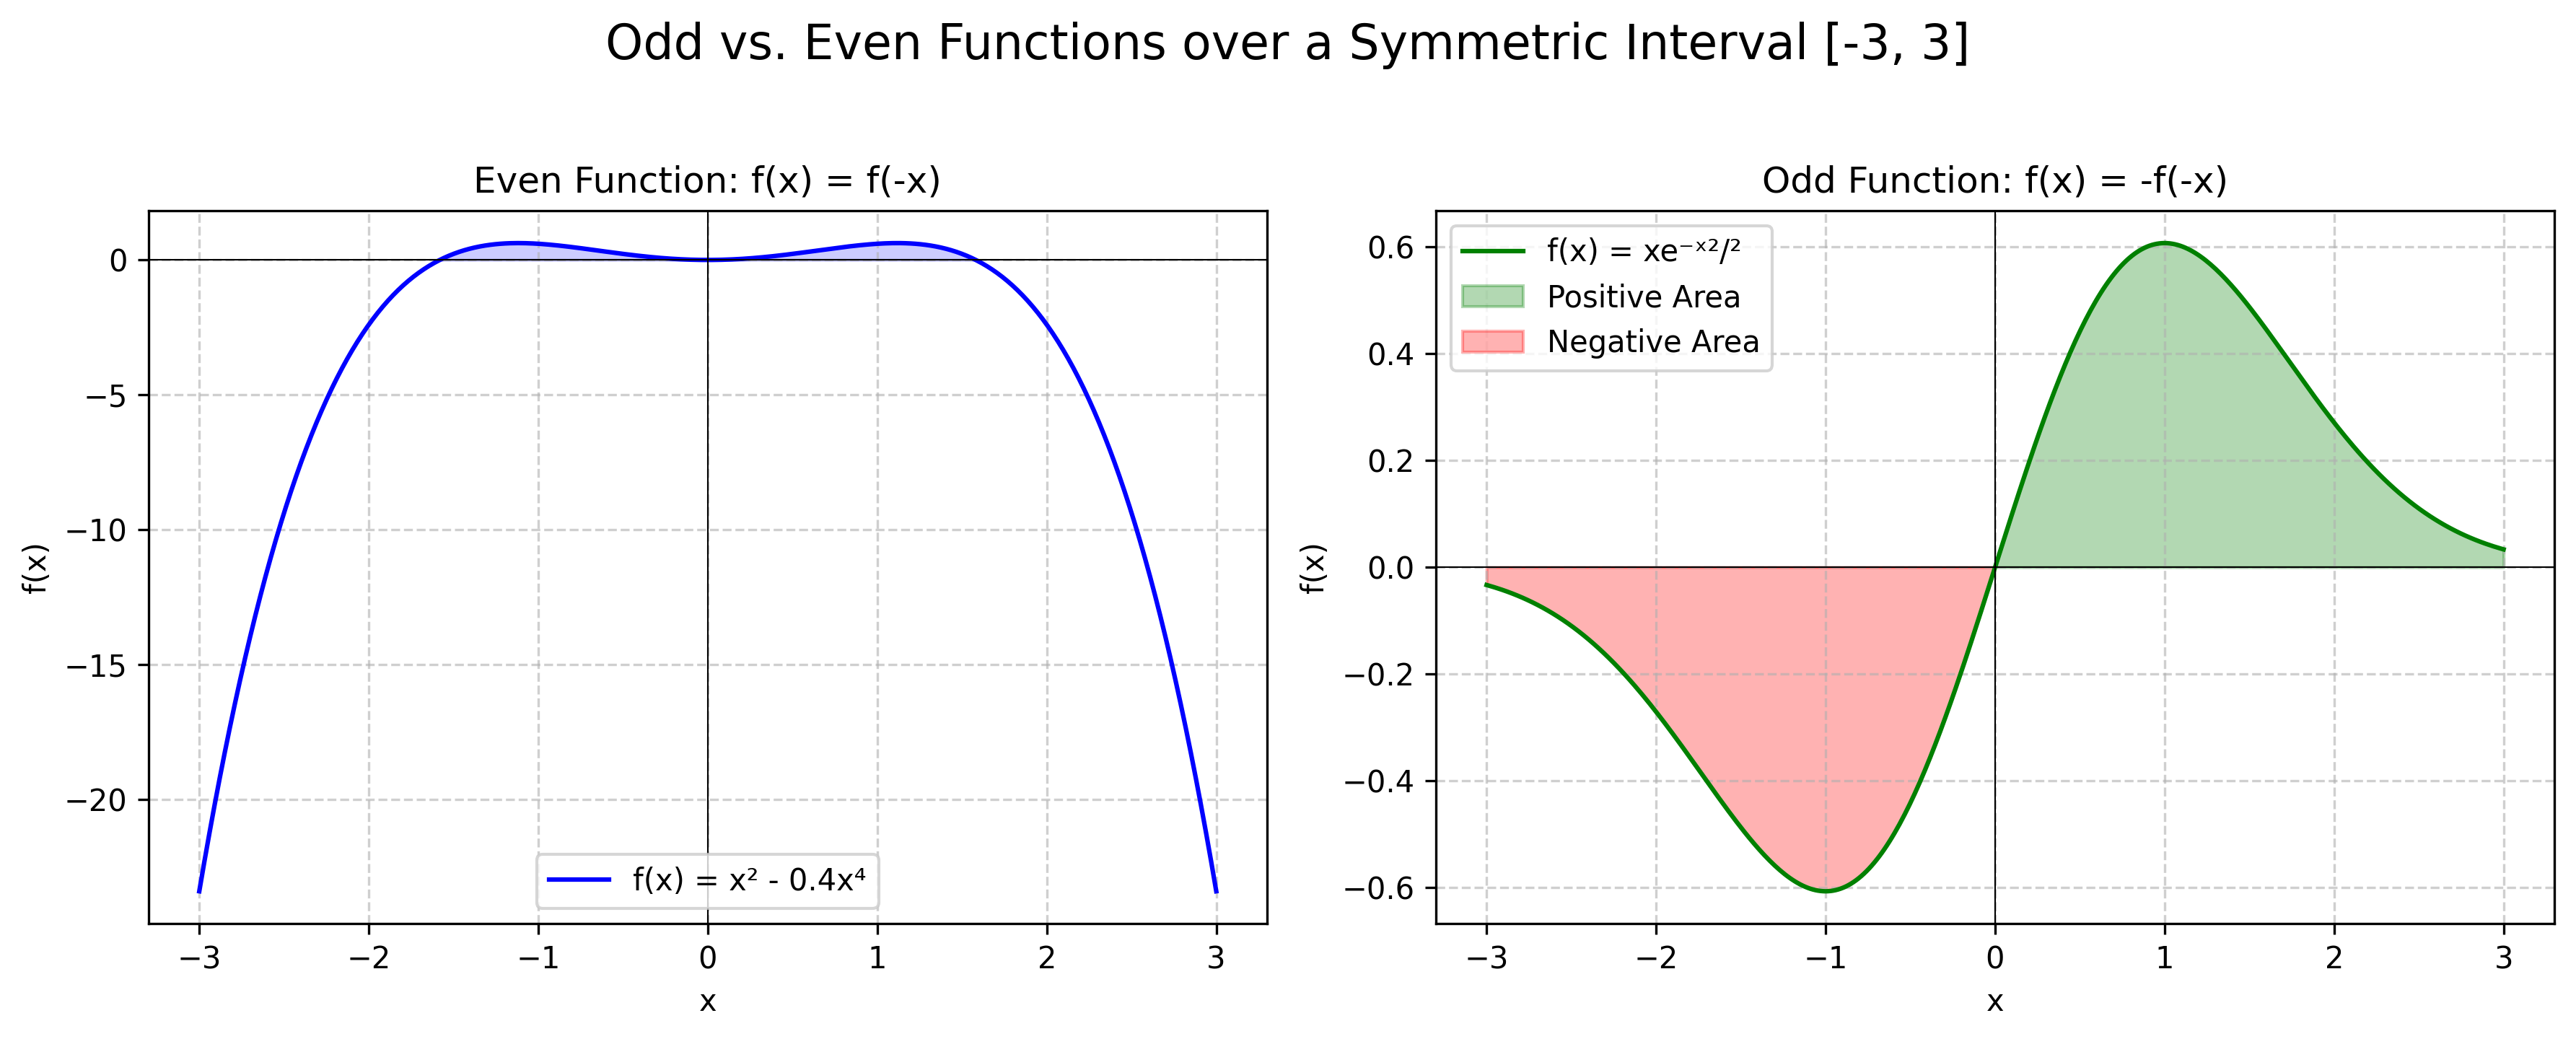
\includegraphics[width=0.8\textwidth]{figure_6_odd_even_functions.png}
  \caption{Odd vs. Even functions over a symmetric interval.}
  \label{fig:odd_even}
\end{figure}

\subsection{Completing the Square}
Used to transform quadratic forms into standard integral forms.
\begin{example}[$\tan^{-1}$ form (Note Example)] $\int \frac{dx}{4x^2+4x+2}$
Complete the square on the denominator:
$4x^2+4x+2 = 4(x^2+x) + 2 = 4(x^2+x+\frac{1}{4}) - 1 + 2 = 4(x+\frac{1}{2})^2 + 1 = (2x+1)^2 + 1$.
The integral becomes $\int \frac{dx}{(2x+1)^2 + 1}$.
Let $u = 2x+1$, $du = 2 dx \Rightarrow dx = du/2$.
\[
\int \frac{du/2}{u^2 + 1} = \frac{1}{2} \int \frac{du}{u^2+1} = \frac{1}{2}\tan^{-1}(u) + C = \frac{1}{2}\tan^{-1}(2x+1) + C
\]
\end{example}

\begin{example}[$\sin^{-1}$ form (Note Example)] $\int \frac{dx}{\sqrt{2x-x^2}}$
Complete the square on the denominator:
$2x-x^2 = -(x^2-2x) = -(x^2-2x+1-1) = -((x-1)^2 - 1) = 1 - (x-1)^2$.
The integral becomes $\int \frac{dx}{\sqrt{1-(x-1)^2}}$.
Let $u = x-1$, $du = dx$.
\[
\int \frac{du}{\sqrt{1-u^2}} = \sin^{-1}(u) + C = \sin^{-1}(x-1) + C
\]
\end{example}

\subsection{The Fundamental Theorem of Calculus}
The FTC links integration and differentiation, and is the formal basis for the relationship between a Probability Density Function (PDF) and a Cumulative Distribution Function (CDF) \cite[Sec 1.3.2]{Chan2021}.

\begin{theorem}[Fundamental Theorem of Calculus \cite{Chan2021}]
Let $f$ be a continuous function on $[a, b]$.
\[
f(x) = \frac{d}{dx} \int_{a}^{x} f(t) dt
\]
\end{theorem}

\begin{example}
Consider $f(t) = t^2$.
The integral from 0 to $x$ is $F(x) = \int_0^x t^2 dt = \left[ \frac{t^3}{3} \right]_0^x = \frac{x^3}{3}$.
The derivative of $F(x)$ is $F'(x) = \frac{d}{dx}\left(\frac{x^3}{3}\right) = x^2$, which is $f(x)$.
\end{example}

\begin{figure}[h!]
  \centering
  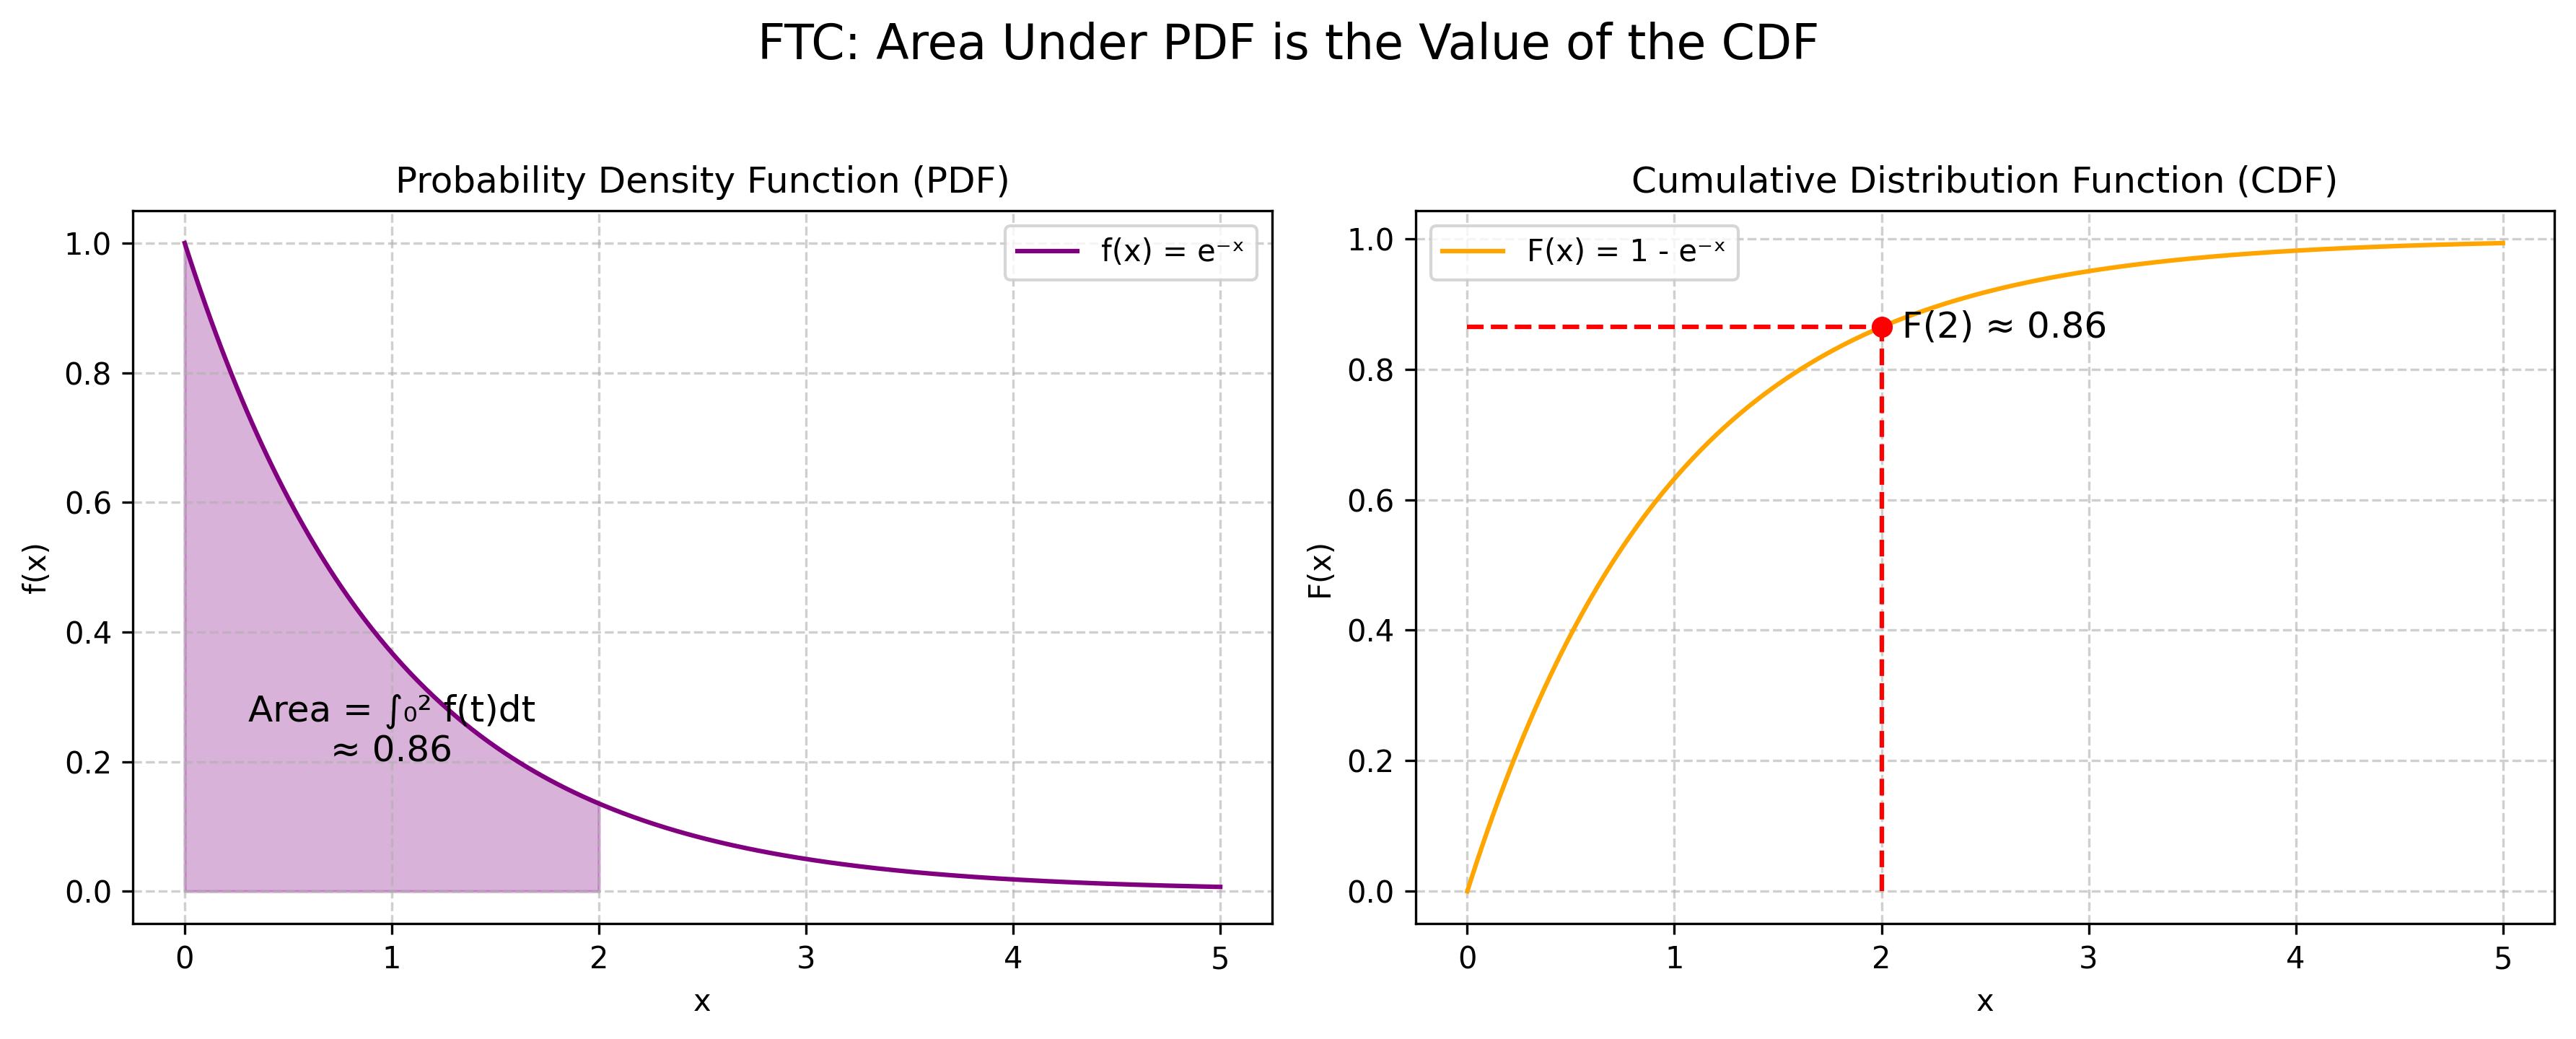
\includegraphics[width=0.8\textwidth]{figure_7_ftc_pdf_cdf.png}
  \caption{Illustration of the FTC via a PDF $f(x)$ and its CDF $F(x) = \int_0^x f(t) dt$.}
  \label{fig:ftc}
\end{figure}

\subsection{The Gaussian Integral}
A famous definite integral that is central to probability and the normal distribution.
\[
I = \int_{-\infty}^{\infty} e^{-x^2} dx = \sqrt{\pi}
\]
\textbf{Proof (using Polar Coordinates):}
\begin{enumerate}
    \item Square the integral and use different dummy variables:
    \[
    I^2 = \left( \int_{-\infty}^{\infty} e^{-x^2} dx \right) \left( \int_{-\infty}^{\infty} e^{-y^2} dy \right) = \int_{-\infty}^{\infty} \int_{-\infty}^{\infty} e^{-(x^2+y^2)} dx dy
    \]
    \item Convert to polar coordinates:
    $x^2 + y^2 = r^2$ and $dx dy = r dr d\theta$.
    The region (entire xy-plane) becomes $r \in [0, \infty)$ and $\theta \in [0, 2\pi)$.
    \[
    I^2 = \int_{0}^{2\pi} \left( \int_{0}^{\infty} e^{-r^2} r dr \right) d\theta
    \]
    \item Solve the inner integral with substitution ($u = r^2, du = 2r dr \Rightarrow r dr = du/2$):
    \[
    \int_{0}^{\infty} e^{-r^2} r dr = \int_{0}^{\infty} e^{-u} \frac{du}{2} = \frac{1}{2} [-e^{-u}]_0^\infty = \frac{1}{2} (0 - (-1)) = \frac{1}{2}
    \]
    \item Solve the outer integral:
    \[
    I^2 = \int_{0}^{2\pi} \left( \frac{1}{2} \right) d\theta = \frac{1}{2} [\theta]_0^{2\pi} = \frac{1}{2} (2\pi) = \pi
    \]
\end{enumerate}
Since $I^2 = \pi$, we have $I = \sqrt{\pi}$.

\textbf{Generalized Gaussian Integral:}
A more general form used in statistics is:
\[
\int_{-\infty}^{\infty} e^{-\alpha x^2} dx = \sqrt{\frac{\pi}{\alpha}}
\]

% --- BIBLIOGRAPHY ---
\bibliographystyle{plain}
\bibliography{references}

\end{document}
% --- END DOCUMENT ---

